\documentclass[]{standalone}  
\usepackage[utf8]{inputenc}
\usepackage[american]{circuitikz}
\usepackage{graphicx}

\renewcommand{\=}{=}

\begin{document}  
    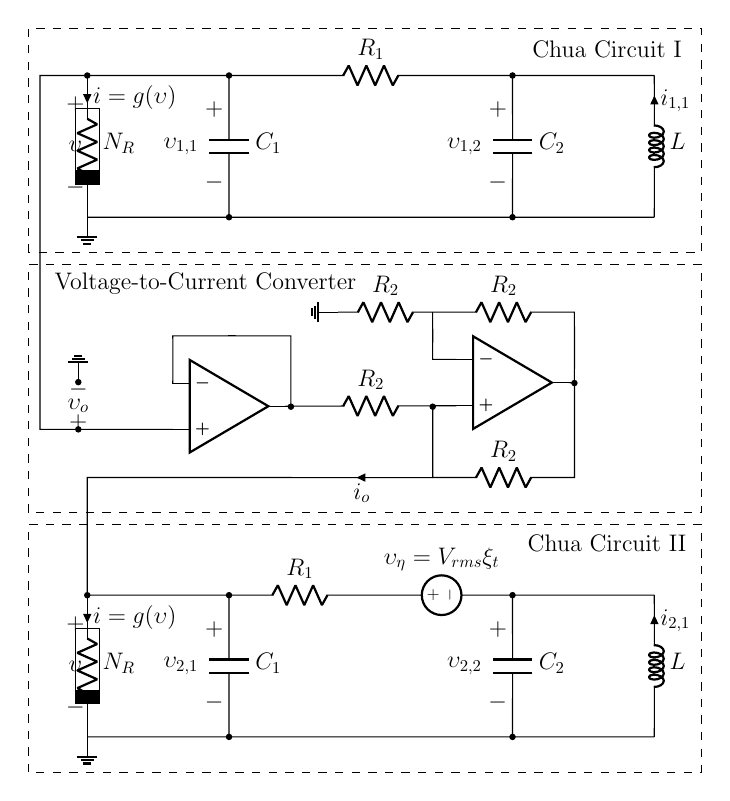
\begin{tikzpicture}[scale=0.6, every node/.style={scale=0.6, font=\Large}]
        \begin{scope}
            \draw (0, 0) node[ground]{} coordinate (o1) to[resistor, l_=$N_R$, i_<=$i \= g(\upsilon)$] ++(0, 3) coordinate(b1);
            \draw (-0.25, 0.25) to[open,v^<=$\upsilon$] (-0.25, 2.75);
            \draw (b1) to[short] ++(3, 0) coordinate(c1);
            \draw (c1) to[resistor, l=$R_1$] ++(6, 0) coordinate(d1);
            \draw (d1) to[short] ++(3, 0) coordinate(e1);
            \draw (c1) to[capacitor, l=$C_1$, v=$\upsilon_{1,1}$, *-*] ++(0, -3);
            \draw (d1) to[capacitor, l=$C_2$, v=$\upsilon_{1,2}$, *-*] ++(0, -3);
            \draw (e1) to[cute inductor, l=$L$, i<=$i_{1,1}$] ++(0, -3) coordinate(f1);
            \draw (o1) -- (f1);
            \draw ([yshift=0.7cm, xshift=-0.25cm] o1) rectangle ([yshift=-0.7cm, xshift=0.25cm] b1);
            \fill ([yshift=0.7cm, xshift=-0.25cm] o1) rectangle ([yshift=-2cm, xshift=0.25cm] b1);
            \draw[dashed] ([yshift=-0.75cm, xshift=-1.25cm] o1) rectangle ([yshift=1cm, xshift=1cm] e1) coordinate (g1);
            \node at ([xshift=-2cm, yshift=-0.45cm] g1){Chua Circuit I};
        \end{scope}
        
        \begin{scope}[shift={(0cm, -5.5cm)}]
            \node at (3, 1.5)[op amp](op1){};
            \node at (9, 2)[op amp](op2){};
            \draw (op1.-) to[short] ++(0, 1) to[short] ++(2.5, 0) to[short, -*] ++(0, -1.5);
            \draw (op1.out) to[resistor, l=$R_2$] (op2.+);
            \draw (op2.-) to[short] ++(-0.5, 0) to[short] ++(0, 1) coordinate (a2);
            \draw (a2) to[resistor, l=$R_2$] ++(3,0) to[short, -*] ++(0,-1.5) coordinate(b2) to (op2.out);
            \draw (b2) to[short] ++(0, -2) to[resistor, l_=$R_2$] ++(-3, 0) coordinate(c2) to[short, -*]++(0, 1.5);
            \draw[dashed] (-1.25, -0.75) rectangle (13, 4.5) coordinate (g2);
            \node at ([xshift=-10.5cm, yshift=-0.4cm] g2){Voltage-to-Current Converter};
            \draw (a2) to[resistor, l_=$R_2$] ++(-2cm, 0cm) node[ground, rotate=-90]{};
        \end{scope}

        \begin{scope}[shift={(0cm, -11cm)}]
            \draw (0, 0) node[ground]{} coordinate (o3) to[resistor, l_=$N_R$, i_<=$i \= g(\upsilon)$, -*] ++(0, 3) coordinate(b3);
            \draw (-0.25, 0.25) to[open,v^<=$\upsilon$,] (-0.25, 2.75);
            \draw (b3) to[short] ++(3, 0) coordinate(c3);
            \draw (c3) to[resistor, l=$R_1$] ++(3, 0) to[voltage source, l=$\upsilon_\eta \= V_{rms} \xi_t$] ++(3,0) coordinate(d3);
            \draw (d3) to[short] ++(3, 0) coordinate(e3);
            \draw (c3) to[capacitor, l=$C_1$, v=$\upsilon_{2,1}$, *-*] ++(0, -3);
            \draw (d3) to[capacitor, l=$C_2$, v=$\upsilon_{2,2}$, *-*] ++(0, -3);
            \draw (e3) to[cute inductor, l=$L$, i<=$i_{2,1}$] ++(0, -3) coordinate(f3);
            \draw (o3) -- (f3);
            \draw ([yshift=0.7cm, xshift=-0.25cm] o3) rectangle ([yshift=-0.7cm, xshift=0.25cm] b3);
            \fill ([yshift=0.7cm, xshift=-0.25cm] o3) rectangle ([yshift=-2cm, xshift=0.25cm] b3);
            \draw[dashed] ([yshift=-0.75cm, xshift=-1.25cm] o3) rectangle ([yshift=1.5cm, xshift=1cm] e3) coordinate (g3);
            \node at ([xshift=-2cm, yshift=-0.4cm] g3){Chua Circuit II};
        \end{scope}
        \draw (c2) to[short, i=$i_o$] ++(-3, 0) -| (b3);
        \draw (b1) to[short, *-] ++(-1, 0) |- (op1.+);

        \draw ([xshift=-2cm] op1.+) to[open, *-*, v=$\upsilon_o$] ++(0, 1cm) node[ground, rotate=180]{};
    \end{tikzpicture}
\end{document} 